\documentclass[12pt]{IEEEtran}
\IEEEoverridecommandlockouts
\usepackage{fancyhdr}
\usepackage{graphicx}
\usepackage[spanish, es-tabla, es-nodecimaldot]{babel}
% \usepackage[utf8]{inputenc}
\usepackage{csquotes}
\usepackage{wrapfig}
\usepackage[l3]{csvsimple}
\usepackage{array}
\usepackage[calc, spanish]{datetime2}
\usepackage{enumitem}
% \usepackage{multicol}
\usepackage{chemformula}
\usepackage{multirow}
\usepackage{mismath}
\usepackage{adjustbox}
\usepackage{nccmath}
\usepackage{amsmath}
\usepackage{amssymb}
\usepackage{mathtools}
\usepackage{amsfonts,latexsym} % para tener disponibilidad de diversos simbolos
\usepackage{enumerate}
\usepackage{empheq}
\usepackage{derivative}
\usepackage{float}
\usepackage{threeparttable}
\usepackage{ifpdf}
\usepackage{rotating}
\usepackage{stfloats}
\usepackage{tabularray}
\usepackage{url}
% \usepackage[inline]{showlabels}
\usepackage{kantlipsum}
\usepackage{siunitx}
\usepackage{makecell}%To keep spacing of text in tables
\setcellgapes{2pt}%parameter for the spacing in tables
\usepackage{afterpage}
\usepackage[
  sorting=none,
  backend=biber,
  style=ieee,
  % bibstyle = authoryear,
  citestyle=numeric-comp,
]{biblatex}
\usepackage{hyperref}
\usepackage{cleveref}
\crefname{table}{tabla}{tablas} % Table's cross-reference name
\crefname{equation}{ec.}{ecs.} %
\newcommand\crefrangeconjunction{--}
\newcommand\crefpairconjunction{~y~}
\providecommand{\abs}[1]{\lvert#1\rvert}
%%%%%%%%%%%%%%%%%%%%%%%%%%%%%%%%%%%%%%%%%%%
%%% CREAR Y REESCRIBIR ALGUNOS COMANDOS %%%
%%%%%%%%%%%%%%%%%%%%%%%%%%%%%%%%%%%%%%%%%%%
\newcolumntype{P}[1]{>{\centering\arraybackslash}p{#1}}  %% Se crea un nuevo tipo de columna llamada P.
\newcommand{\tabitem}{~~\llap{\textbullet}~~}
\newcommand{\ctt}{\centering\scriptsize\textbf} %%\ctt abrevia el comando \centering\scriptsize\textbf
\newcommand{\dtt}{\scriptsize\textbf} %%\dtt abrevia el comando \scriptsize\textbf
\renewcommand\IEEEkeywordsname{Palabras clave}

%% Crea una lista en dos columnas
\SetEnumitemKey{twocol}{%
  itemsep = 1\itemsep,
  parsep = 0.5\parsep,
  before = \raggedcolumns
  \begin{multicols}{2},
    after =
\end{multicols}}
%%%%%%%%%%%%%%%%%%%%%%%%%%%%%%%%%%%%%%%%%%%

% correct bad hyphenation here
\hyphenation{op-tical net-works semi-conduc-tor} %% Con este comando se especifican como pueden seprarse las sílabas adecuadamente en caso una palabra quede en dos lineas diferentes de texto

\graphicspath{ {figs/} {logos/}}  %%Ruta donde se encuentran las imágenes, que esté vacio indica que las imagenes están dentro de la misma carpeta que contiene el archivo .tex

\sisetup{
  output-decimal-marker = {.},
  uncertainty-mode = separate,
}
% adjust as needed
\addtolength{\footskip}{0\baselineskip}
\addtolength{\textheight}{-1\baselineskip}

%Paquete tikz para hacer diagramas y figuras
\usepackage{tikz}
\usetikzlibrary{arrows}
%\usepackage[spanish,es-noquoting]{babel}

%%%%%%%%%%%%%%%%%%%%%%%%%%%%%%%%
%%%%% INICIO DEL DOCUMENTO %%%%%
%%%%%%%%%%%%%%%%%%%%%%%%%%%%%%%%

\addbibresource{CaracterizacionPeliculaDelgadaAluminioHiPIMSTribologia.bib}

\DTMsavedate{duedate}{2024-03-25}% Año-Mes-Día -> Fecha de entrega
\DTMnewdatestyle{usvardate}{%
  \renewcommand{\DTMdisplaydate}[4]{%
    \DTMMonthname{##2}\nobreakspace% Mes
    \number##1% Año
  }%
  \renewcommand{\DTMDisplaydate}{\DTMdisplaydate}%
}

\DeclareSIUnit{\min}{min}

\begin{document}
%%%%%%%%%%%%%%%%%%%%%%%%%%%%
%%% TÍTULO DEL DOCUMENTO %%%
%%%%%%%%%%%%%%%%%%%%%%%%%%%%

\title{Análisis de plasma de nitruro de boro (\ch{BN}) por espectrometría de emisión óptica obtenido por RF Magnetron Sputtering}

%%%%%%%%%%%%%%%%%%%%%%%%%%%
%%%%%%%%% AUTORES %%%%%%%%%
%%%%%%%%%%%%%%%%%%%%%%%%%%%
\author{\IEEEauthorblockN{Jesús Diego Gómez Garnica, Marcos López Merino}\\
	\IEEEauthorblockA{\textbf{Profesor}: Julio César Cruz Cárdenas}\\
	\IEEEauthorblockN{\DTMusedate{duedate}}}

%%%%%%%%%%%%%%%%%%%%%%%%%%%
\twocolumn[
	\begin{@twocolumnfalse}
		\maketitle
		\begin{abstract}
			En este trabajo se estudió la composicion del plasma emitido por un deposito de boro por el metodo RF (magnetron sputtering), analizando el espectro de emision a una altura de 5 cm por encima del blanco y en el centro del mismo, por intervalos de tiempo para concretar una base de datos para su posterior analisis, donde estudiando estas franjas de emision, se obtuvieron elementos tales como Nitrogeno, Argon y Boro, presenten en el deposito de la camara de vacío.

		\end{abstract}

		\begin{IEEEkeywords}
			Espectometria, RF magnetron sputtering, Plasma
		\end{IEEEkeywords}
	\end{@twocolumnfalse}
	\vspace{1cm}
]

%https://doi.org/10.1016/j.surfcoat.2022.128409 -> Aplicaciones

%%%%%%%%%%%%%%%%%%%%%%
%\IEEEpeerreviewmaketitle
%%%%%%%%%%%%%%%%%%%%%%%%%%%%%%%%%%%%%
%%% PRIMERA SECCIÓN DEL DOCUMENTO %%%
%%%%%%%%%%%%%%%%%%%%%%%%%%%%%%%%%%%%%
\section{Introducción}

Las películas delgadas son capas muy finas de material, con espesores que van desde unos pocos nanómetros hasta micrómetros. Estas películas tienen aplicaciones en electrónica, óptica, recubrimientos protectores y más.

En la historia moderna de la física, se han creado diversos métodos para construir estas estructuras que conocemos como películas delgadas, por mencionar algunas tenemos electrodeposición (\emph{electroplating}), la evaporación, la pulverización catódica (\emph{sputter deposition}), la deposición química de vapor  (CVD, por sus siglas en inglés) y combinaciones de estas. Sin embargo, la técnica utilizada en ese trabajo es la llamada RF.

Sputtering RF \cite{mastertesis2017}: La pulverización catódica por radio frecuencia (RF) ocurre a frecuencias superiores a 50 kHz. En esta, los iones no alcanzan suficiente movilidad como para establecer una descarga similar a la del sputtering DC y los electrones tienen suficiente energía como para causar colisiones ionizantes en el espacio entre los electrodos, lo que produce el plasma en el espacio entre los electrodos. Una de las mayores ventajas de usar sputtering RF es que se pueden utilizar blancos no conductores, pues se aplica un potencial oscilante en el blanco, lo que hace que en cada medio ciclo se puedan acelerar los iones del plasma hacia la superficie con suficiente energía como para producir la pulverización catódica y en el otro medio ciclo, los electrones del plasma alcanzan la superficie, impidiendo cualquier tipo de acumulación de carga. Las frecuencias RF usadas para la deposición por sputtering están en el rango de 0.5 y 30 MHz siendo 13.56 MHz la frecuencia más usada comercialmente. Una de las mayores desventajas de la pulverización catódica de materiales semiconductores o aislantes es que la mayoría de estos materiales tienen baja conductividad térmica, grandes coeficientes de expansión térmica y son usualmente materiales frágiles, y este tipo de propiedades son indeseables en un proceso como el RF sputtering donde la mayoría de la energía de bombardeo produce calor y se generan grandes gradientes de temperatura en el blanco, lo que puede producir su fractura.

En este sentido, al ser Boro un material dieléctrico, se buscó esta alternativa de RF para la fabricación de la película delgada; no obstante, el enfoque de este escrito no es acerca del producto de este método, sino del plasma generado por el mismo.

Los plasmas \cite{plasmaaaaa} se generan suministrando energía a un gas neutro, lo que provoca la formación de portadores de carga. Los electrones e iones se producen en fase gaseosa cuando electrones o fotones con suficiente energía colisionan con los átomos y moléculas neutros del gas de alimentación (ionización por impacto electrónico o fotoionización). Existen diversas maneras de suministrar la energía necesaria para la generación de plasma a un gas neutro en este caso a través de RF. La generación de un plasma mediante el uso de haces de partículas cargadas, especialmente electrones, y de haces de fotones se analizará al final, a través de espectrómetro de emisión óptica.

\section{Procedimiento experimental}

Para el procedimiento se inició por depositar un blanco de boro de 5 pulgadas de diámetro, para posteriormente formar una película delgada sobre un sustrato en este caso de vidrio (porta objetos) con una presión de 20 $\mu Torr$ y un foto sensor, que capte las emisiones de radiación justo al frente de la cámara de vació, como se muestra en la \ref{fig:Espectometro}   


\begin{figure}[htp]
	\centering
	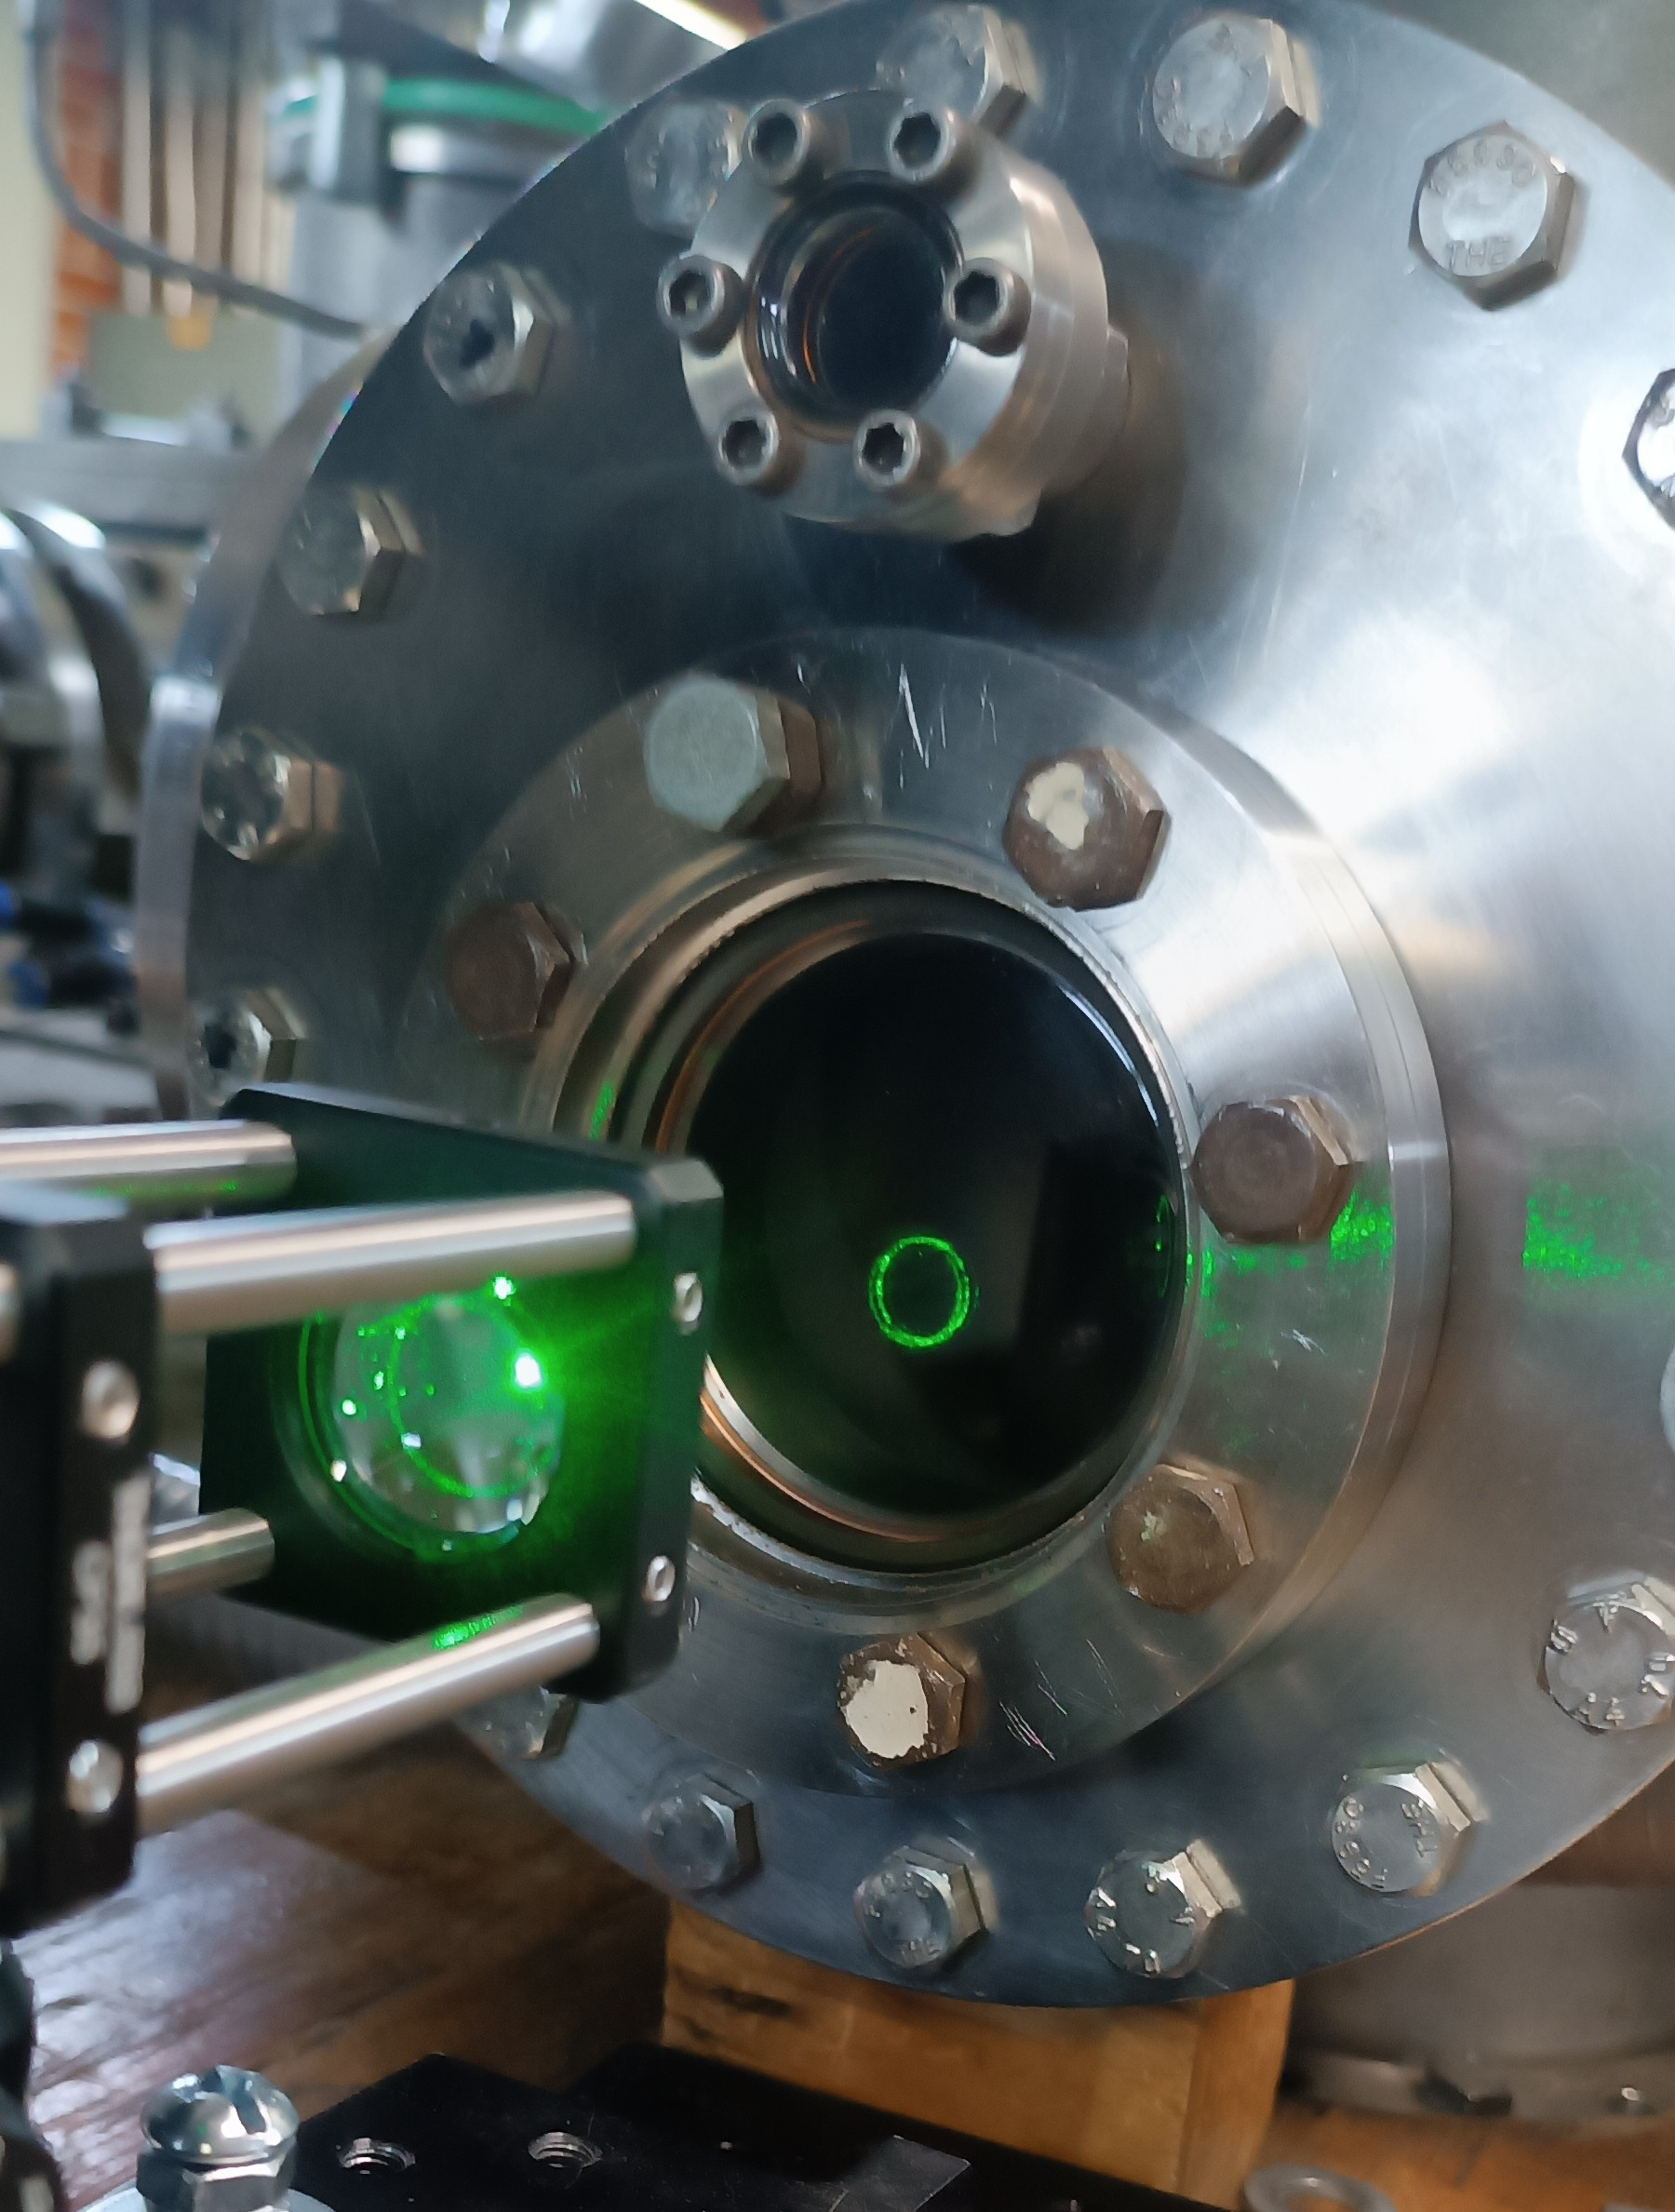
\includegraphics[width=0.6\linewidth]{figs/buenaaaaaaaaa.jpg}
	\caption{Espectrómetro óptico enfocado en el centro del blanco de Boro.}
	\label{fig:Espectometro}
\end{figure}

\subsection{Medición de Espectros}

Para la medición de los espectros de emisión, este espectrómetro se colocó enfocado en el centro del blanco de Boro, a una altura de 5 cm por encima del mismo, este centro se vario cada 0.2 mm y se obtuvieron los datos respectivos de emisión, variando 2 cm a ambos lados de lo que se ubicó como el centro del blanco, la duración total del deposito fue de 20 minutos, dando por resultado el plasma que se se observa en \ref{fig:plasma}

\begin{figure}[htp]
	\centering
	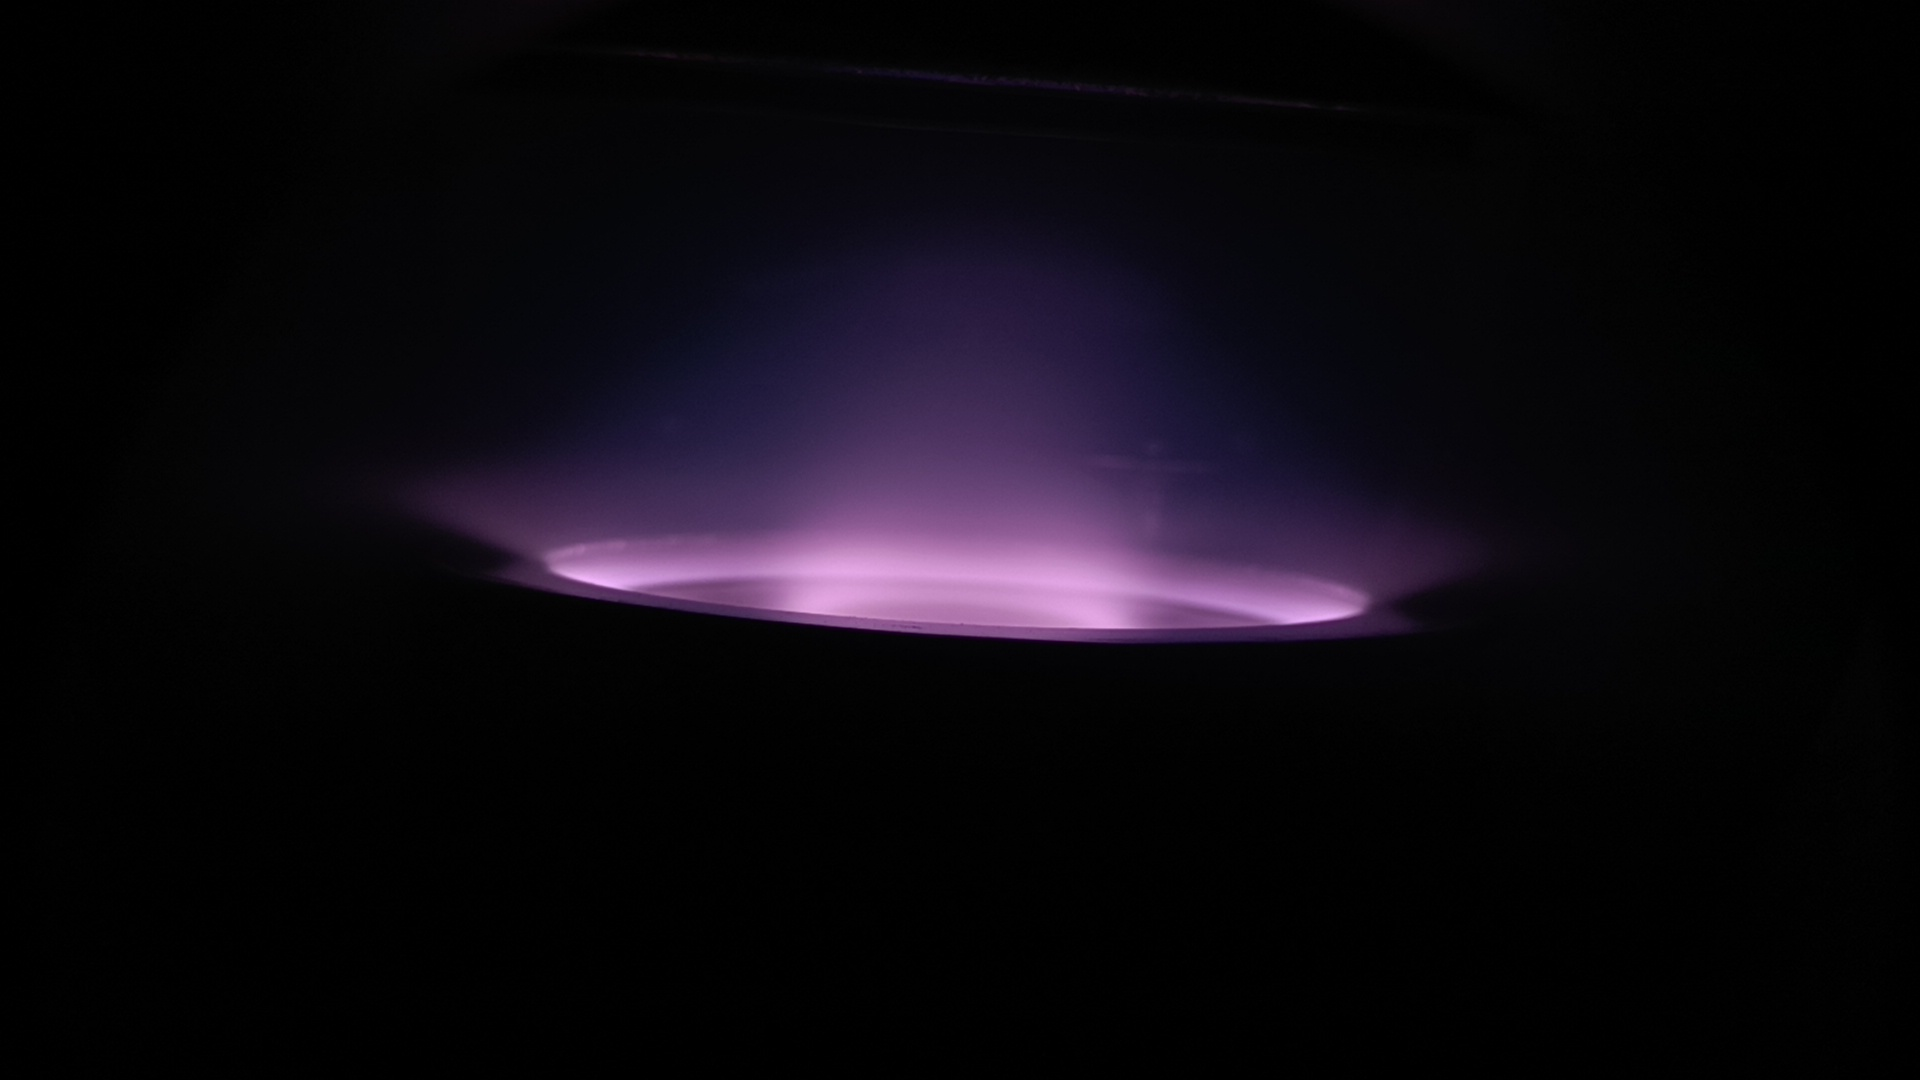
\includegraphics[width=0.8\linewidth]{figs/PLASMA.jpg}
	\caption{Plasma generado por deposito de un blanco de Boro por el metodo de RF.}
	\label{fig:plasma}
\end{figure}

\section{Resultados y análisis}

Una vez obtenida una gama de mediciones de los espectros de emisión  de diferentes posiciones alrededor del centro del blanco se procedió a comparar las lineas de emision obtenidas con las de National Institute of Standards and Technology Atomic Spectra Database, es importante aclarara que las longitudes de onda que captaba en espectometro optico variaba de $200 nm $ a $900 nm$.

\begin{figure}[htp]
	\centering
	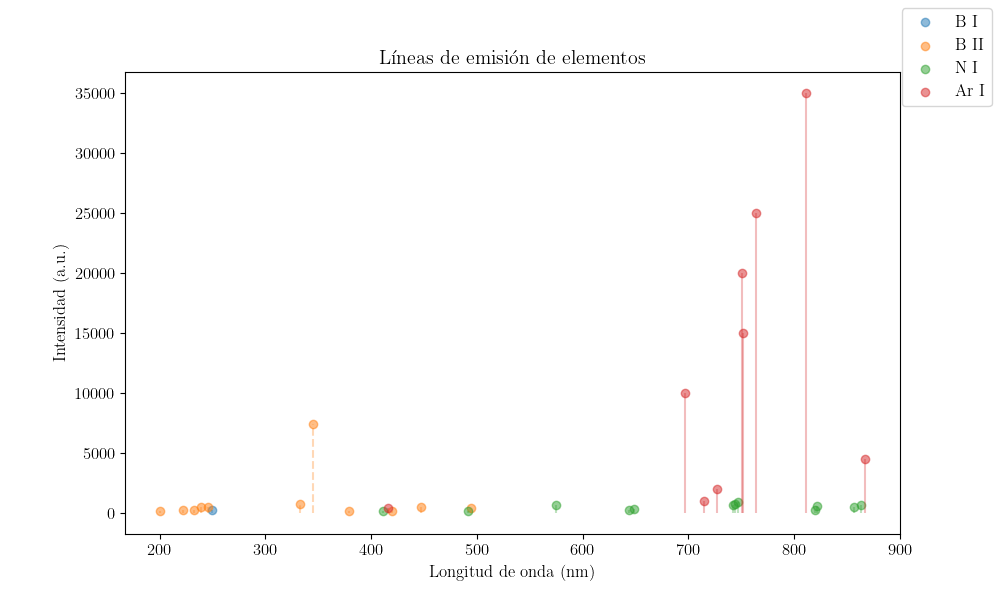
\includegraphics[width=0.9\linewidth]{descarga.png}
	\caption{Comparacion de los espectros de emision teoricos y obtenidos en el laboratorio.}
	\label{Graf:plasma}
\end{figure}

Principalmente se identificaron las franjas de emisión de BI, BII, N y Ar, que es lo que esperaríamos del deposito encontrado, sin embargo, los datos obtenidos presentaban bastante ruido, esto se tomo en cuenta a la hora de filtrar, se esperaba encontrar otro elemento como el oxigeno, pues aunque este deposito se hace en una cámara de vacío, la extracción total del oxigeno presente en el aire es complicado de lograr, esto se le puede atribuir a movimientos en la mesa óptica y un cristal de la cámara de vació deteriorado pudieron afectar estas mediciones.


\section{Conclusiones}
El plasma es toda una área de la física por explorar y entender, se puede aprender bastante de su estudio para futuras aplicaciones principalmente en los temas relacionados con la Astrofísica, en este sentido al explorar los elementos en conjunto con un plasma generado nos 



%%%%%%%%%%%%%%%%%%%%%%%%%%%%%%%%
%%%%%%    Bibliografia   %%%%%%%
%%%%%%%%%%%%%%%%%%%%%%%%%%%%%%%%
% \newpage
\nocite{*}
\printbibliography
%\section{Apéndices}
%\appendices
\end{document}
%%%%%%%%%%%%%%%%%%%%%%%%%%%%%%%%
%%%%%% FIN DEL DOCUMENTO %%%%%%%
%%%%%%%%%%%%%%%%%%%%%%%%%%%%%%%%
